\documentclass[11pt]{article}



% Packages
\usepackage[utf8]{inputenc}
\usepackage{amsmath}    % For math equations
\usepackage{graphicx}   % For including images
\usepackage{geometry}   % For page layout
\usepackage{hyperref}   % For hyperlinks
\usepackage{enumitem}   % For custom lists
\usepackage{cite}       % For better citations

\usepackage[style=ieee,backend=bibtex]{biblatex}
\addbibresource{references.bib}  % This line loads your bibliography file

% Page Layout
\geometry{a4paper, margin=1in}

% Title and Author Information
\title{\textbf{A Comparative Study of Deep Learning Models for Fruit Classification in Low-Data Scenarios}}

\author{
    Ankit Sapkota, Nischal Ojha, Sanjeev Kumar Shah, Yogendra Baskota \\[6pt]
    \textit{Department of Electronics and Computer Engineering} \\ 
    \textit{Pashchimanchal Campus, Tribhuvan University, Nepal} \\[6pt]
    \texttt{ankitsapkotaquartz@gmail.com, nischalojha59@gmail.com,} \\[6pt]
    \texttt{ sahsanjeev42@gmail.com,yogendrabaskota18@gmail.com} \\[6pt]
}

\date{\today}

% Begin Document
\begin{document}

% Title
\maketitle
\thispagestyle{empty}  % Remove page number from title page

% Abstract
\renewcommand{\abstractname}{\Large Abstract}

\begin{abstract}
\vspace{8pt}
 Segregating rotten fruits from fresh ones is a significant challenge faced by the fruit industry, critical for maintaining quality and reducing waste. In this research, we explore the application of deep learning models for fruits classification and identify effective methods for separating rotten fruits from fresh ones. Our study evaluates the performance of two state of the art pretrained models, ResNet and EfficientNet, alongside a small custom neural network tailored for this task in small dataset scenario of 3 fruit types, we analyze the models based on accuracy, precision, and recall. The ResNet and Efficient model achieved the accuracy of 99\% and surprisingly our custom model achieved the accuracy of 97\%.In this paper, detailed comparison is conducted among them. \cite{paper1}
\end{abstract}


\noindent \textbf{Keywords:} Deep learning, ResNet, EfficientNet, Custom neural network, Fruit industry.

%\vspace{16pt} % Adds some space after the keywords
%\hrule % Creates a horizontal line


% Sections of your document
\section{Introduction}
%We’re in the fast-evolving era of Machine Learning \& Artificial Intelligence. Deep Learning plays a key part in the evolution of machine learning. Deep Learning can be used in the fields like Automatic Speech Recognition (ASR), Image Recognition, Natural Language Processing, Drug Discovery and Toxicology, Customer Relationship Management, Recommendation Systems and Bioinformatics \cite{intro1}. With its increasing study, more application areas of deep learning are being discovered. One classical problem of machine learning and machine vision is image classification.\cite{intro2} 

%Fruit classification\cite{methodology2} is a significant piece of work in the agro-food industries. To separate the rotten fruits from fresh and good ones and minimize wastage, the accuracy of detection of rotten fruits is important. Doing so, the quality standards are ensured. In the recent years, deep learning models are known for remarkable success in tasks like image classification tasks \cite{intro2} which makes them a promising solution for fruit classification challenges.

%Despite the high potential of deep learning models, they are extremely data-hungry as they demand large amount of labeled data to achieve a well-behaved performance model \cite{intro3}. Acquiring such large labeled datasets for fruit classification can be labor-intensive and cost expensive. To address such issue, techniques like transfer learning, data augmentation and the use of pre-trained models can be done. 

Deep learning has shaped many industries, tremendously contributing in delivering much needed insights with much cheaper running cost. It is playing pivotal role in transforming many industries including Segregation. 
Segregating fruits is the pivotal element in fruit supply pipeline, higher efficiency at this part ensures the quality of fruit supply. Precisely identifying ripeness level of fruits at scale can help assist scheduling the time of fruit supply.
Image based classification using deep learning\cite{intro2} models has shown promising signs to automate this process, but with the wide variety of fruits and difference in texture, shape and whole outlook of even the same exact fruit grown in different part of the world pose a significant challenge to this solution.
Small amount of data is available to train these data hungry models \cite{intro3}, data scarce solutions must be posed to cater solution in the existing status quo, our research dives into the evaluation of various deep learning models and their performance in fruit classification in data scarce scenario.




%The aim of this study is to build and evaluate deep learning models for classifying rotten fruits from fresh ones. The goal is to compare the performance of models, to identify the most effective one in low-data scenarios. 

%The results of this research are expected to contribute to the development of reliable, and efficient solutions for fruit classification. 
%The remainder of this paper is organized as follows: Section 2 presents the methodology and dataset used in the study, Section 3 discusses the experimental results, and Section 4 concludes with the findings and future directions. (To be done at last.) 


%\section{Related Work}
%Deep Residual Learning for Image Recognition\cite{paper1} introduced ResNet to handle the vanishing gradient problem in deep neural networks with skip connections. By allowing the training of very deep architectures, ResNets achieved state-of-the-art performance on benchmark image recognition tasks such as ImageNet and significantly improved classification accuracy.

\section{Methodology}
We are using two state-of-art architectures along with our small custom neural network for the purpose of classification of rotten fruits with fresh ones. We fine-tuned the pre-trained models for transfer learning\cite{methodology1} and trained our small custom neural network which is trained from scratch for the specific purpose of classification. Datasets containing images of different fruits is collected and different models are trained on that same dataset. After training and fine-tuning those models, we found that transfer learning from those pretrained models helped in increasing the performance in all datasets but surprisingly our small custom neural network was also able to achieve similar performance for same datasets.
\subsection{Models}
%We are using ResNet-18 and EfficientNet-b0 as pretrained models, both of them are popular in transfer learning for image classification\cite{methodology2,methodology3}. ResNet-18 is used in various fields along with classification of fruits\cite{methodology4,methodology5,methodology6}. EfficientNet has been found even more effective than ResNet for image classification\cite{methodology7}. We freeze the last layer of both pretrained models for fine-tuning purpose and built custom layer. We also designed our custom neural network with the basic building block as popular sequence of 2D convolution and has 3 repetitions of basic layer. 


To lay the groundwork for our study, we select multiple neural network architectures and evaluate their performance. We train both standard, high performing IMAGENET architectures that have been popular for transfer learning, as well as a family of significantly smaller convolutional neural networks. For the standard IMAGENET architectures, we evaluate ResNet-18 \cite{model1-11} and efficientNet-b0 \cite{model2}, which have both been used extensively in transfer learning applications. We also design or custom simple and small convolutional architectures, The basic building block for this is the popular sequence of a (2d) convolution, followed by batch normalization \cite{model3} and a relu activation. Our custom neural network consists three repetition of this.


\subsection{Dataset}
Our primary dataset, banana consist of banana images collected by Webcam of ASUS ZENBOOK 14X OLED, of specification 1080p, mixed with data collected by Sultana et al of specification 1111*1590 along and other internet images. Images of Apple and Oranges were taken form the dataset by Sultana et al \cite{dataset1}  mixed with internet images. All the images were resized to 256*256 before training. Each fruit contained two categories including rotten and fresh, rotten fruits generally had patches or stain on  the skin.


\begin{figure}[h]
    \centering
    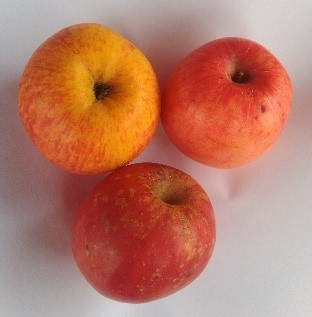
\includegraphics[width= 0.14\textwidth]{images/app.jpg} 
    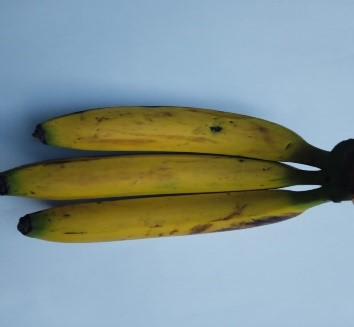
\includegraphics[width= 0.153\textwidth]{images/ban.jpg} 
    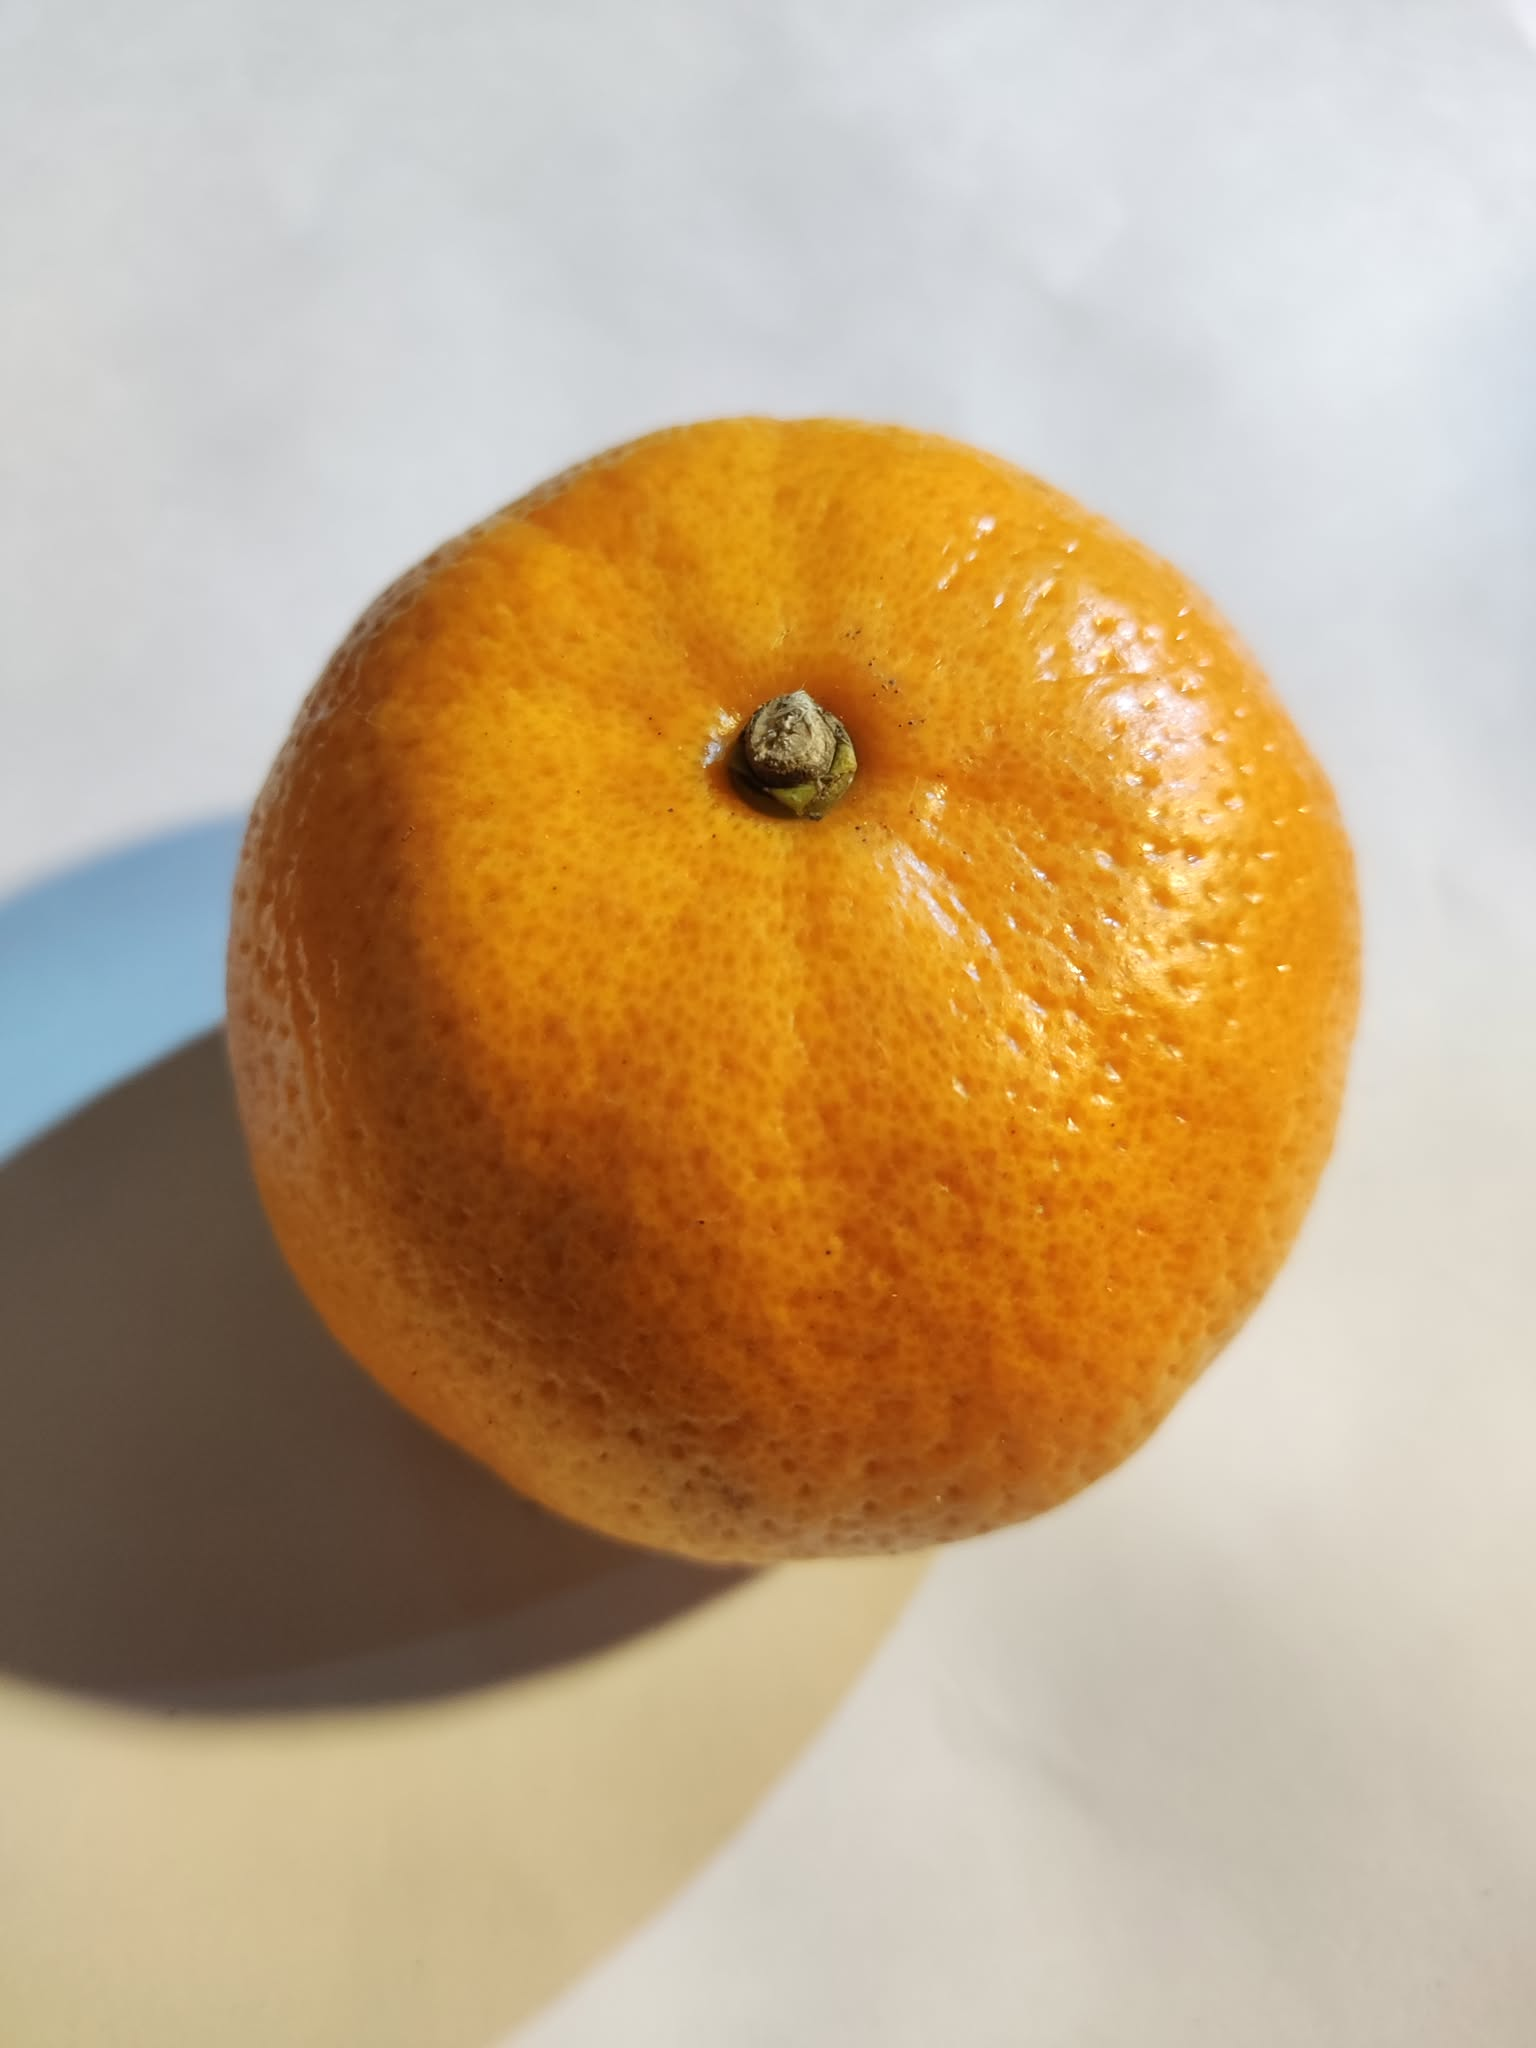
\includegraphics[width= 0.105\textwidth]{images/freshorange.jpg} 
    \caption{Fresh Fruits samples}
    \label{fig:example_label}
\end{figure}

\begin{figure}[h]
    \centering


    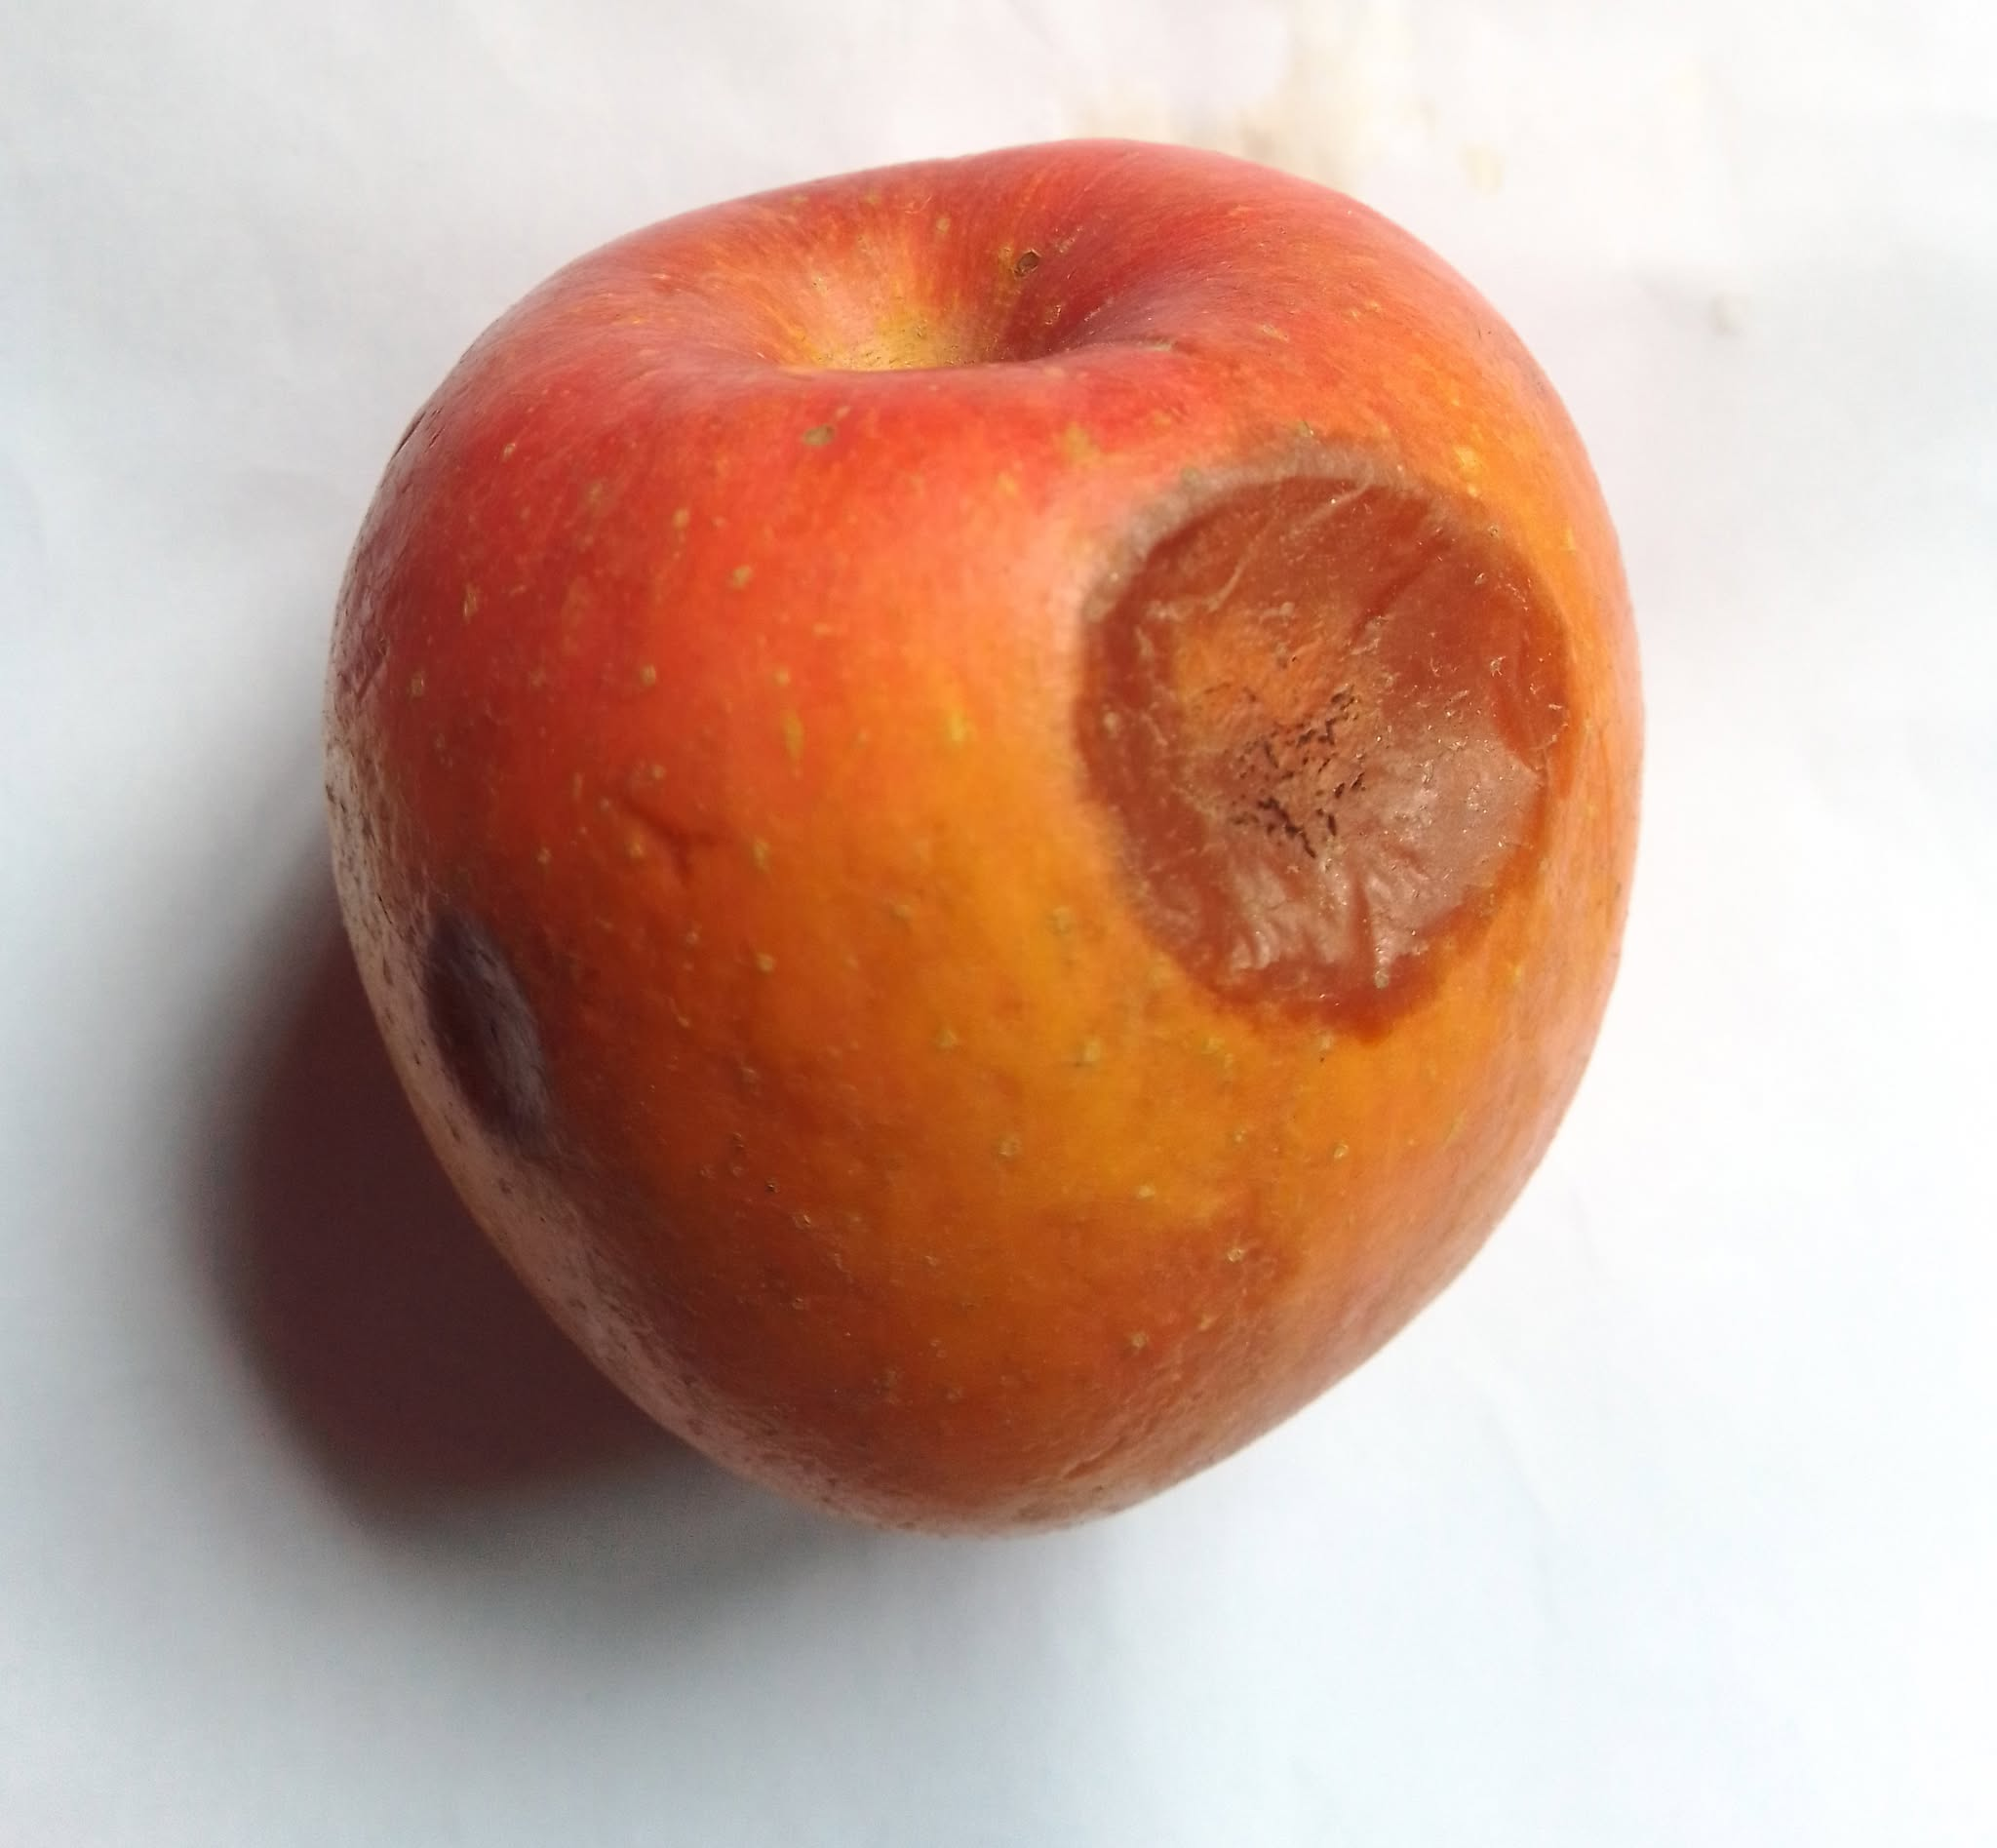
\includegraphics[width= 0.145\textwidth]{images/rottenapple.jpg} 
    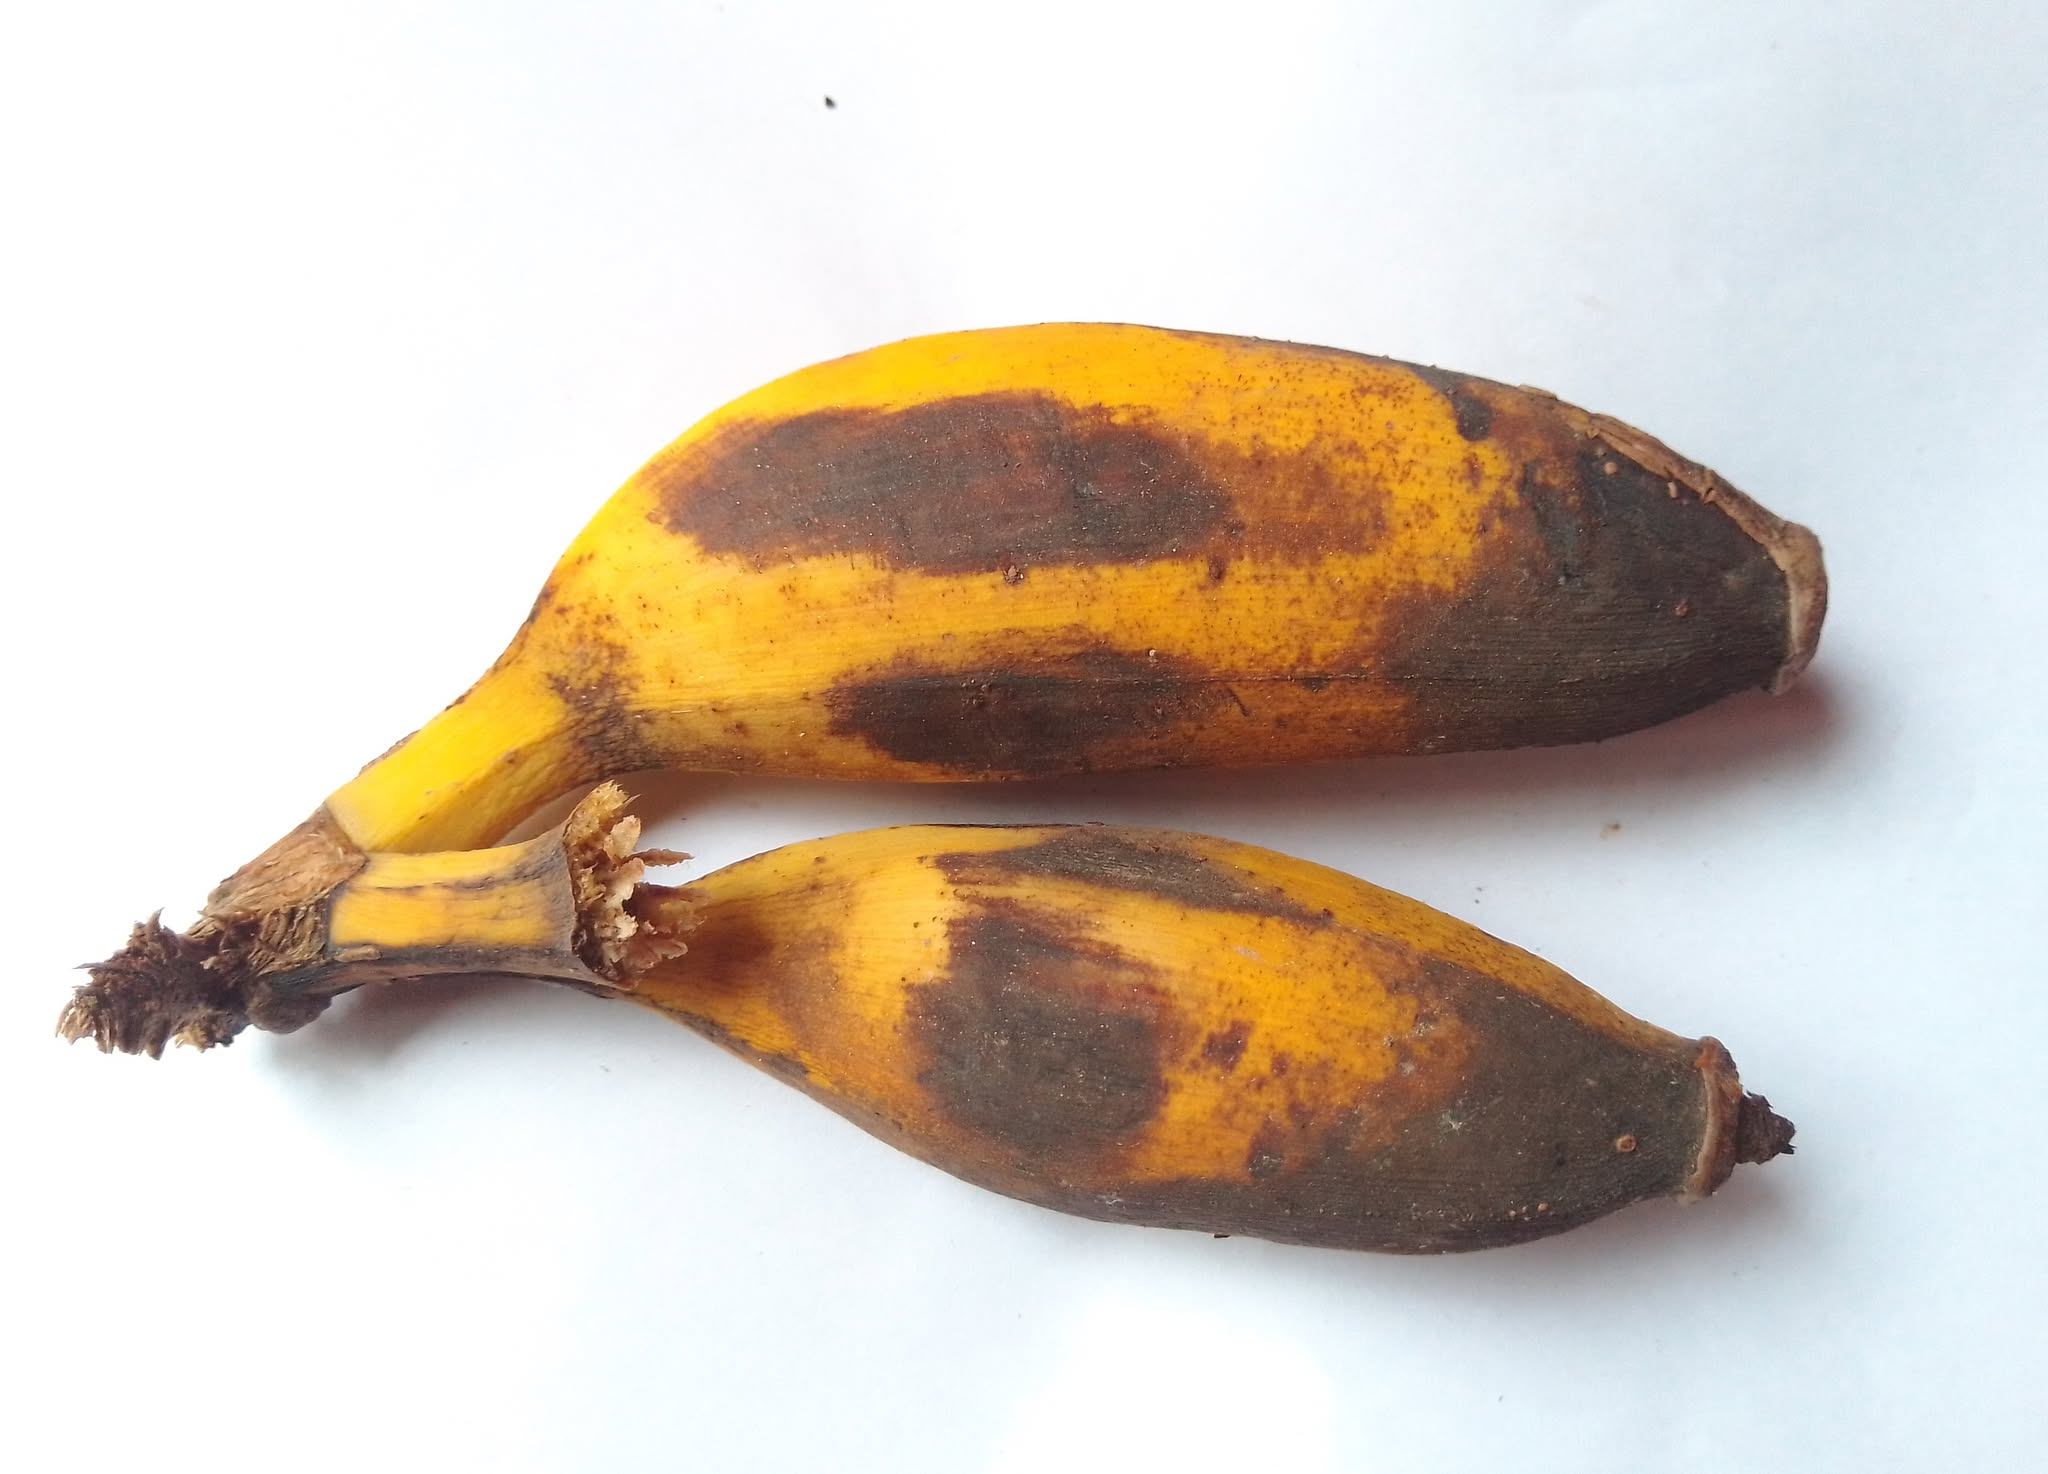
\includegraphics[width= 0.19\textwidth]{images/rottenbanana.jpg}    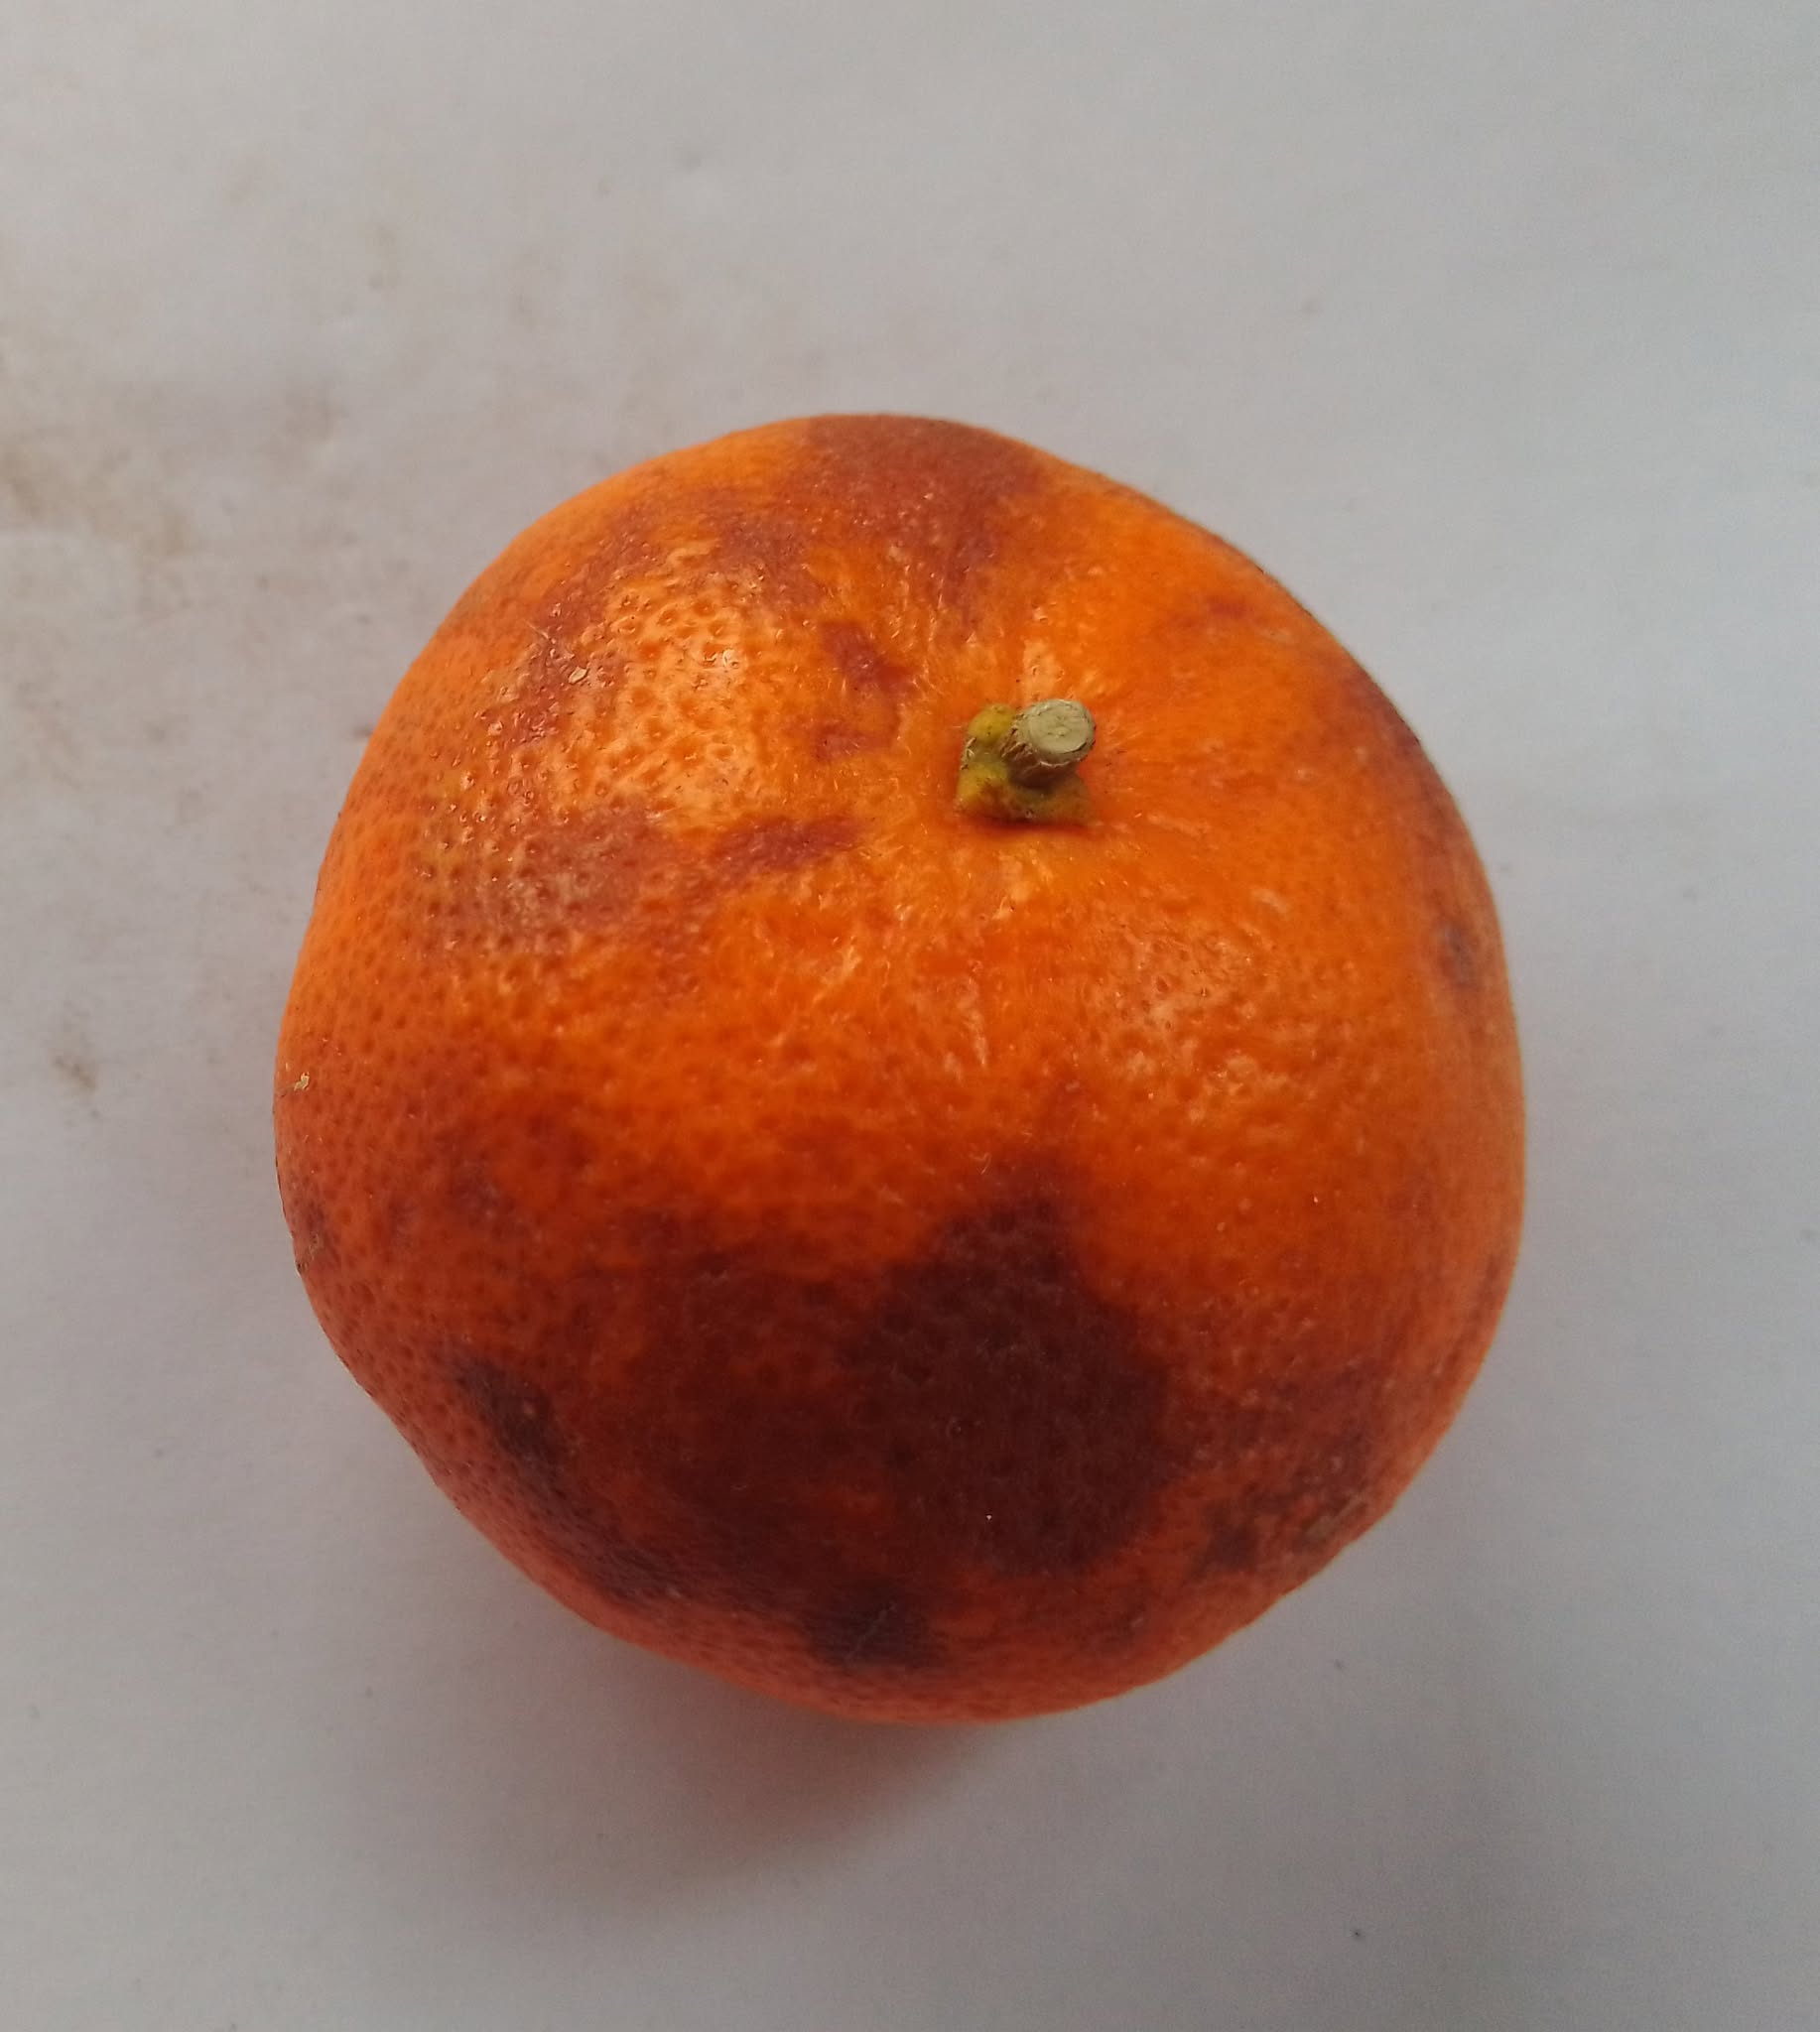
\includegraphics[width= 0.122\textwidth]{images/rottenorange.jpg} 
    \caption{Rotten Fruits samples}
    \label{fig:example_label}
\end{figure}



\section{Results}
We find that across all datasets and all models, transfer learning does not significantly affect performance. Additionally, our lightweight convolutional networks performs comparably to standard IMAGENET models. 
While IMAGENET architecture quickly attain maximum accuracy within few epochs, our custom network took comparatively more epochs before it reach its maximum. 
%\subsection{Research Findings}

\textbf{Following table shows the result of our research}




\begin{table}[ht]
\centering
\resizebox{\textwidth}{!}{%
\begin{tabular}{|*{10}{c|}}
\hline

\multicolumn{1}{|c|}{\textbf{Fruits}} & \multicolumn{3}{|c|}{\textbf{ResNet}} & \multicolumn{3}{|c|}{\textbf{EfficientNet}} & \multicolumn{3}{|c|}{\textbf{CNN}} \\ \hline
Apple & Accuracy  & Precision & Recall & Accuracy & Precision & Recall & Accuracy & Precision & Recall  \\ \hline
Apple & 98.14\%  & 98.16\% & 98.14\% & 98.06\% & 98.06\% & 98.09\% & 97.95\% & 98.03\% & 98.01\%  \\ \hline
Banana & 99.34\% & 99.34\% & 99.34\% & 99.02\% & 99.02\% & 99.02\% & 98.32\% & 98.37\% & 98.32\% \\ \hline
Orange & 98.94\% & 98.95\% & 98.94\% & 98.43\% & 97.02\% & 97.00\% & 97.01\% & 99.01\% & 99.02\% \\ \hline
\end{tabular}%
}

\caption{Research Findings}
\label{tab:customtable}
\end{table}


%\subsubsection{Evaluation of Research Finding}


The small difference in result between our small Convolutional neural network and Imagenet Models would have arise from the fact that IMAGENET architectures have a large number of parameters concentrated at the higher layers, for this reason, the design of these models is likely to be suboptimal for the this application and our task start with an image of a bodily region of interest and use variations in local textures to identify rotten ones. For example, in banana images, black patches are the indication of rotten banana, This contrasts with natural image datasets like IMAGENET, where there is often a clear global subject of the image. Similar results were found with medical images.\cite{transfusion}





\section{Conclusion}
While comparing various deep learning models the ResNet and Efficient model achieved the highest accuracy but surprisingly our custom model also achieved the accuracy close to imgenet. We find that transfer learning offers limited performance gains and much smaller architectures can perform comparably to the standard IMAGENET models.
% Print the bibliography or references
\printbibliography
\end{document}
